\chapter{Manipulando GUI}

O PD foi desenvolvido utilizando um modelo que separa a apresentação das
funcionalidades.
Isto rola com 2 linguagens de programação: C para a engine e tcl/tk para as GUI.
GUI e engine se comunicam por um socket que permite, inclusive, que a engine
do PD seja executada em uma máquina e a GUI em outra.
Apesar de não ser intenção de ensinar Tcl/tk, passaremos uma visão geral desta
linguagem.

% \url{http://puredata.info/docs/guiplugins/GuiPluginsAPI/}

% -----+-----+-----+-----+-----+-----+-----+-----+-----+-----+-----+-----+-----+
%      |     |     |     |     |     |     |     |     |     |     |     |     |
% -----+-----+-----+-----+-----+-----+-----+-----+-----+-----+-----+-----+-----+
\section{Iniciando no Tcl/Tk - Hello World}
O Tcl (Tool Command Language) é uma linguagem de programação dinâmica bastante
poderosa e simples de ser utilizada. 
Tk é um conjunto de ferramentas para construção de GUI de aplicações desktop e é
a GUI padrão não apenas do TCL mas de várias outras linguagens e pode ser
executada nativamente em vários sistemas operacionais modernos como Windows, Mac
OS X, Linux, entre outros \footnote{Visite: http://www.tcl.tk/ para maiores
informações}.

O Tk possui vários objetos prontos para GUI como botões, labels, janelas,
checkbox, entre outros.
Os objetos criados devem ser armazenados em uma variável.
Toda variável em Tk possui um nome que inicia com ponto (\texttt{.}) e devem ser declaradas
de maneira hierárquica.
O ponto (.) defina a aplicação principal.
Se a mesma possuir um canvas, por exemplo, este pode ser chamado \texttt{.canvas}.
Se neste canvas for adicionado uma reta, a mesma pode ser chamadta \texttt{.canvas.reta}
e assim sucessivamente.
Após criar o objeto e definir seus atributos, basta que o mesmo seja empacotado
(\texttt{pack}).

\begin{lstlisting}[caption=Exemplo de Hello World]
label .hello -text "Hello World"
pack .hello
\end{lstlisting}

Uma vez que um programa tk esteja pronto, basta salvá-lo com a extensão .tcl e
utilizar um interpretador para executá-lo.
Um exemplo deste interpretador no Linux é o wish. Assim, salvando o exemplo anterior com o nome de helloWorld.tcl e executando

\begin{lstlisting}[caption=Executando o Hello World]
wish helloWorld.tcl
\end{lstlisting}

Teremos o resultado:
\begin{figure}[ht!]
	\centering
	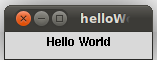
\includegraphics[scale=\Mysize]{helloWorld}
	\caption{Hello World no Tcl/Tk}
\end{figure}

No diretório tk deste tutorial temos exemplos mais interessantes de GUI com Tk
mas a prática desta linguagem vai além do escopo deste tutorial.
Um tutorial mais completo de Tcl/Tk pode ser encontrado em 
\footnote{http://www.bin-co.com/tcl/tutorial/} e uma lista dos objetos e
parâmetros pode ser encontrada em\footnote{http://www.tkdocs.com/widgets/index.html}.

% -----+-----+-----+-----+-----+-----+-----+-----+-----+-----+-----+-----+-----+
%      |     |     |     |     |     |     |     |     |     |     |     |     |
% -----+-----+-----+-----+-----+-----+-----+-----+-----+-----+-----+-----+-----+
\section{Executando comandos Tcl/tk no PD}

Para testarmos o funcionamento dos comandos tcl no PD, é possível utilizarmos o
TCL Prompt.
No Pure Data Vanila o mesmo se encontra no Menu Help > TCL Prompt.

Também fizemos um \external que possibilita executar comandos tcl no PD.
Diferentemente do editor do PD, nosso \external aceita algumas variáveis
de substituição como, por exemplo, canvas.
Adiante explicaremos o porquê desta substituição ser necessária.

\begin{figure}[ht!]
	\centering
	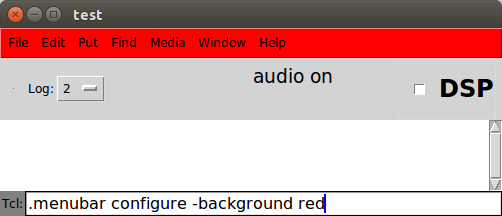
\includegraphics[scale=\Mysize]{tcl_prompt}
	\caption{Prompt tcl como \external}
\end{figure}

% -----+-----+-----+-----+-----+-----+-----+-----+-----+-----+-----+-----+-----+
%      |     |     |     |     |     |     |     |     |     |     |     |     |
% -----+-----+-----+-----+-----+-----+-----+-----+-----+-----+-----+-----+-----+
\section{Alterando a GUI do PD}
Os objetos do pd podem ser alterado pelo console TCL.

\begin{lstlisting}[Exemplo de alteração de menus do PD com Tcl]
.menubar configure  -foreground black

wm title .pdwindow test
\end{lstlisting}

Uma maneira de verificar  todos os filhos da janela do PD

\begin{lstlisting}
foreach c [winfo children .pdwindow] {puts [winfo name $c]}

.menubar.file
.menubar.edit
.menubar.put
.menubar.media
.menubar.window
.menubar.help

.pdwindow.text
.pdwindow.text.internal

.pdwindow.header.dsp
.pdwindow.header.loglabel
.pdwindow.header.dio configure -foreground red

.pdwindow.tcl.label
.pdwindow.tcl.entry

.aboutpd

\end{lstlisting}

Para verificar todos os filhos da aplicação principal

\begin{lstlisting}
foreach c [winfo children .] {puts [winfo name $c]}
\end{lstlisting}
Isto irá listar todas as janelas do PD.
Com isto, é possível alterar a janela

\begin{lstlisting}
wm title .x12be7d0 test
\end{lstlisting}

O padrão do PD utiliza nomeia o canvas como .c

Assim, dá para mudar a cor do canvas com 

\begin{lstlisting}
.x12be7d0.c configure -bg blue
\end{lstlisting}

Verifique o arquivo pdwindow.tcl no código-fonte.

\begin{figure}[ht!]
	\centering
	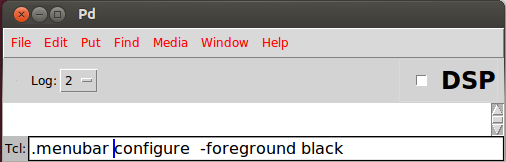
\includegraphics[scale=\Mysize]{menubar}
	\caption{Alterando a cor da barra de menus}
\end{figure}

\begin{figure}[ht!]
	\centering
	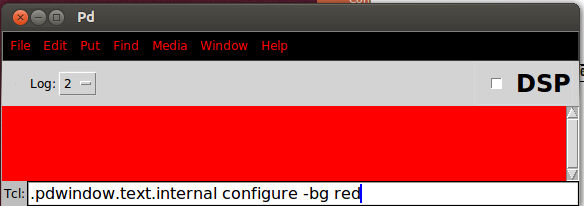
\includegraphics[scale=\Mysize]{text_internal}
	\caption{Alterando a cor do console}
\end{figure}

\begin{lstlisting}[caption=Escrevendo no console]
::pdwindow::verbose 1 "Hello, World!\n"
::pdwindow::verbose 0 "Hello, World!\n"
::pdwindow::error "Houston, we have a problem!\n"
::pdwindow::fatal "See you on the other side.\n"
::pdwindow::post  "This message will self destruct in five seconds.\n"
::pdwindow::debug "Second phase initiated\n"
\end{lstlisting}

\begin{figure}[ht!]
	\centering
	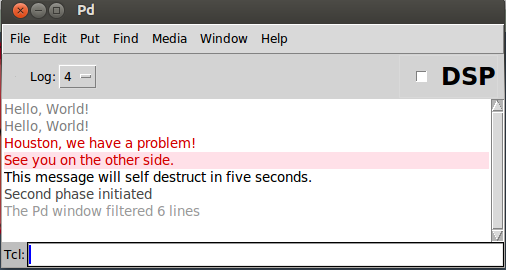
\includegraphics[scale=\Mysize]{console}
	\caption{Escrevendo no console}
\end{figure}

% -----+-----+-----+-----+-----+-----+-----+-----+-----+-----+-----+-----+-----+
%      |     |     |     |     |     |     |     |     |     |     |     |     |
% -----+-----+-----+-----+-----+-----+-----+-----+-----+-----+-----+-----+-----+
\section{Desenhando no canvas}

A tela do Pure Data é um objeto \texttt{canvas} do TCL.
Por esta razão, podemos criar diversos componentes gráficos.

O nome do objeto canvas

Usando tags para mover e apagar.

\begin{lstlisting}
.x12be7d0.c create rectangle 10 10 20 20 -tags my_rectangle

.x12be7d0.c create text 400 200 -text Hello

.x12be7d0.c create oval 100 100 30 50

.x12be7d0.c create polygon 0 0 30 100 50 20 100 50 10 34

.x12be7d0.c create arc 0 0 100 200

.x12be7d0.c create line 0 0 10 10 12 5 15 3 20 12

.x12be7d0.c create image 100 100 -image [image create photo -file /home/flavio/Pictures/csound.gif] -anchor nw
\end{lstlisting}

\begin{figure}[ht!]
	\centering
	
\includegraphics[scale=\Mysize]{canvas_draw}
	\caption{Desenhando no canvas}
\end{figure}

Ou usando variável

\begin{lstlisting}
set im1 [image create photo -file /home/flavio/Pictures/csound.gif]

.x12be7d0.c create image 0 0 -image $im1 -anchor nw
\end{lstlisting}

O canvas permite ainda outras coisas como, por exemplo, gerar uma impressão
(arquivo post script) do mesmo.

\begin{lstlisting}
.x86b880.c postscript -file testdump.ps
\end{lstlisting}

% -----+-----+-----+-----+-----+-----+-----+-----+-----+-----+-----+-----+-----+
%      |     |     |     |     |     |     |     |     |     |     |     |     |
% -----+-----+-----+-----+-----+-----+-----+-----+-----+-----+-----+-----+-----+
\section{Adicionando novos menus}

Adicionar novo item a um menu existente

\begin{lstlisting}
.menubar.edit add command -label blob -command { puts teste } -accel "$mod+J"

bind all <$::modifier-Shift-Key-Z> {menu_redo}

.menubar add  separator

menu .menubar.align

.menubar add cascade -label Align -menu .menubar.align

.menubar.align add command -label Left -command {puts Left}


Inserindo na posicao 

.menubar insert 3 cascade -label Align -menu .menubar.align

.menubar.edit insert 3 command -label  test  -command {puts x} -state disabled

bind <<Loaded>> {menubar.edit entryconfigure test -state enabled}
\end{lstlisting}

% -----+-----+-----+-----+-----+-----+-----+-----+-----+-----+-----+-----+-----+
%      |     |     |     |     |     |     |     |     |     |     |     |     |
% -----+-----+-----+-----+-----+-----+-----+-----+-----+-----+-----+-----+-----+
\section{Internacionalizando plugins}

\begin{lstlisting}
[_ "Save"]
\end{lstlisting}


% -----+-----+-----+-----+-----+-----+-----+-----+-----+-----+-----+-----+-----+
%      |     |     |     |     |     |     |     |     |     |     |     |     |
% -----+-----+-----+-----+-----+-----+-----+-----+-----+-----+-----+-----+-----+
\section{Adicionando widgets ao canvas}

Exemplos adaptados do site: \url{http://pages.cpsc.ucalgary.ca/~saul/personal/archives/Tcl-Tk_stuff/tcl_examples/}

Mais informações\footnote{\url{http://wiki.tcl.tk/490}}

% ------------------------------------------------------------------------------
\subsection{Label}

\begin{lstlisting}
label .x196c840.l1 -text "This is what the default label looks like"
label .x196c840.l2 -text "This is a yellow label on a blue background" \
    -foreground Yellow \
    -background Blue
label .x196c840.l3 -text "This is a label in Times 24 font" \
    -font {-family times -size 24}\
    -bg white

.x196c840.c create window 10 20 -window .x196c840.l1
.x196c840.c create window 10 40 -window .x196c840.l2
.x196c840.c create window 10 60 -window .x196c840.l3
\end{lstlisting}

% ------------------------------------------------------------------------------
\subsection{Button}

\begin{lstlisting}
set text Hello
proc doIt {widget} {
    global text
    if {$text == "Hello"} {
        set text "Goodbye"
    } else {
        set text "Hello"
    }
    $widget configure -text $text
}

button .x196c840.b1 -text "Hello" \
        -command "doIt .x196c840.b1"
button .x196c840.b2 -text "Quit" \
    -command "destroy ."

.x196c840.c create window 10 100 -window .x196c840.b1
.x196c840.c create window 50 100 -window .x196c840.b2
\end{lstlisting}

Atenção! Veja o que acontece quando se pressiona o botão Quit!

url{http://www.tcl.tk/man/tcl8.4/TkCmd/button.htm}
% ------------------------------------------------------------------------------
\subsection{Checkbuttons e RadioButtons}

\begin{lstlisting}
set font helvetica

proc applyIt { } {
    global bold italics font
    if {$bold} {set weight bold} {set weight normal}
    if {$italics} {set slant italic} {set slant roman}
    .x22c0840.c.b configure -font "-family $font -weight $weight -slant $slant"
}

checkbutton .x22c0840.c.c1 -text Bold -variable bold   -anchor w
checkbutton .x22c0840.c.c2 -text Italics -variable italics  -anchor w

radiobutton .x22c0840.c.r1 -text Helvetica -variable font -value helvetica
radiobutton .x22c0840.c.r2 -text Courier   -variable font -value courier   

button .x22c0840.c.b -text Apply \
    -command "applyIt"

applyIt

.x22c0840.c create window 10 100 -window .x22c0840.c.c1
.x22c0840.c create window 110 100 -window .x22c0840.c.c2
.x22c0840.c create window 10 150 -window .x22c0840.c.r1
.x22c0840.c create window 110 150 -window .x22c0840.c.r2
.x22c0840.c create window 10 200 -window .x22c0840.c.b

\end{lstlisting}

% ------------------------------------------------------------------------------
\subsection{Entry}

\begin{lstlisting}
entry .x1b2c3d0.c.es4 -width 3 -textvar S(out) -state readonly

.x1b2c3d0.c create window 490 175          -window .x1b2c3d0.c.es4
\end{lstlisting}

% ------------------------------------------------------------------------------
\subsection{Scale}
\todo{rever}
\begin{lstlisting}
scale .x12b87f0.c.s01 -from 100 -to 0 -label "x" -command {puts }

.x12b87f0.c create window 20 20 -window .x12b87f0.c.s01
\end{lstlisting}

Interessante o fato de o parâmetro ser passado automaticamente para o comando
selecionado.

% ------------------------------------------------------------------------------
\subsection{Spinbox}

\begin{lstlisting}
spinbox .x25d2220.c.sp -from 0.00 -to 5.00 -increment 0.25 -format %5.2f -width 10 \
    -font 10 -justify center -textvariable var -command {::pdwindow::post  "This message will self destruct in five seconds.\n"}
.x25d2220.c create window 20 20 -window .x25d2220.c.sp
\end{lstlisting}

% ------------------------------------------------------------------------------
\subsection{Text}

\begin{lstlisting}
text .x25d2220.c.t -yscrollcommand ".x25d2220.c.t.scroll set" -setgrid true \
        -width 40 -height 10 -wrap word
scrollbar .x25d2220.c.t.scroll -command ".x25d2220.c.t yview"
.x25d2220.c create window 100 20 -window .x25d2220.c.t
\end{lstlisting}
\url{http://www.tcl.tk/man/tcl8.4/TkCmd/text.htm}

% ------------------------------------------------------------------------------
\subsection{Listbox}

\begin{lstlisting}
scrollbar .x25f29b0.c.listbox.s -command ".x25f29b0.c.listbox yview"
listbox .x25f29b0.c.listbox -yscroll ".x25f29b0.c.listbox.s set"

bind .x25f29b0.c.listbox <Double-B1-ButtonRelease> {::pdwindow::post [.x25f29b0.c.listbox get active]}

.x25f29b0.c create window 100 100 -window .x25f29b0.c.listbox
\end{lstlisting}

% ------------------------------------------------------------------------------
\subsection{Choose Color}

\begin{lstlisting}
proc doIt {widget} {
    set current_color \
        [tk_chooseColor -title "Choose a background color" -parent .]
    $widget configure -background $current_color
}
button .x25d2220.c.b -text "Choose a color..." \
        -command "doIt .x25d2220.c"
.x25d2220.c create window 20 400 -window .x25d2220.c.b
\end{lstlisting}

% ------------------------------------------------------------------------------
\subsection{Choose File}

\begin{lstlisting}
set types {
        {"All Source Files"     {.tcl .c .h}    }
        {"Image Files"          {.gif}          }
        {"All files"            *}
}

proc doIt {label} {
    global types   
    set file [tk_getOpenFile -filetypes $types -parent .]
    $label configure -text $file
}

label .x25d2220.c.label -text "No File"
button .x25d2220.c.button -text "Select a file?" \
        -command "doIt .x25d2220.c.label"

.x25d2220.c create window 20 20 -window .x25d2220.c.button
.x25d2220.c create window 20 40 -window .x25d2220.c.label
\end{lstlisting}

% ------------------------------------------------------------------------------
\subsection{Message box}

\begin{lstlisting}
proc doIt {label} {
    set button \
        [tk_messageBox \
               -icon question \
               -type yesno \
               -title Message \
               -parent . \
               -message "Do you like me so far?"]
    $label configure -text $button
}

label .x25d2220.c.label1 -text "I'm not sure yet"
button .x25d2220.c.button1 -text "Do you like me?" \
        -command "doIt .x25d2220.c.label1"

.x25d2220.c create window 20 80 -window .x25d2220.c.button1
.x25d2220.c create window 20 110 -window .x25d2220.c.label1
\end{lstlisting}

% -----+-----+-----+-----+-----+-----+-----+-----+-----+-----+-----+-----+-----+
%      |     |     |     |     |     |     |     |     |     |     |     |     |
% -----+-----+-----+-----+-----+-----+-----+-----+-----+-----+-----+-----+-----+
\section{Eventos}

Como adicionar binds

\url{http://www.tcl.tk/man/tcl8.4/TkCmd/bind.htm}

Fazer uma barra de status com posição x,y
%      sys_vgui("bind .x%lx.c <Motion> {+::pdwindow::post \" %%x %%y\n\"}\n", canvas);

\begin{figure}[ht!]
	\centering
	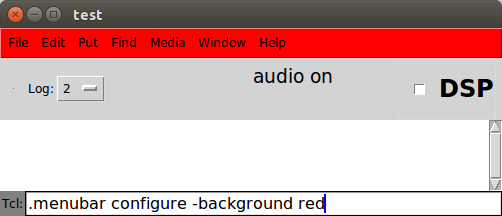
\includegraphics[scale=\Mysize]{tcl_prompt}
	\caption{Prompt tcl como \external}
\end{figure}

\begin{figure}[ht!]
	\centering
	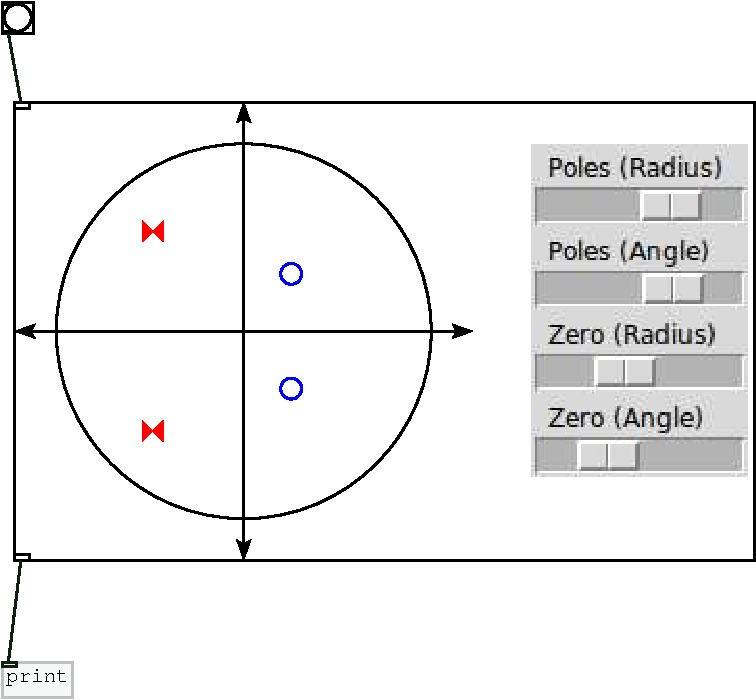
\includegraphics[scale=\Mysize]{filter_circle}
	\caption{Exemplo de \external com GUI TCL}
\end{figure}


% -----+-----+-----+-----+-----+-----+-----+-----+-----+-----+-----+-----+-----+
%      |     |     |     |     |     |     |     |     |     |     |     |     |
% -----+-----+-----+-----+-----+-----+-----+-----+-----+-----+-----+-----+-----+
\section{Trocando dados entre C e TCL}

\begin{lstlisting}
   sys_gui(" if { [catch {pd}] } {proc pd {args} {pdsend [join $args " "]}}\n");
\end{lstlisting}

